% FENG 498 Final Project Report - Warehouse Layout Optimization
% Izmir University of Economics, Industrial Engineering
% Build: pdflatex main.tex (x3)  or  bash build.sh
\documentclass[12pt,a4paper]{article}

\usepackage[utf8]{inputenc}
\usepackage[T1]{fontenc}
\usepackage{mathptmx}                 % Times New Roman look
\usepackage[a4paper,margin=2.5cm]{geometry}
\usepackage{setspace}
\onehalfspacing
\usepackage{graphicx}
\usepackage{booktabs}
\usepackage{makecell}
\usepackage{array}
\usepackage{amsmath}
\usepackage{amssymb}
\usepackage{siunitx}
\usepackage[font=small,labelfont=bf]{caption}
\usepackage{float}
\usepackage{enumitem}
\setlist{topsep=2pt,itemsep=1pt}
\usepackage{xcolor}
\definecolor{covertitle}{RGB}{31,78,121}
\usepackage[hidelinks]{hyperref}

\setcounter{secnumdepth}{3}
\setcounter{tocdepth}{3}
\graphicspath{{figs/}}

\captionsetup[table]{position=above,skip=6pt}
\captionsetup[figure]{position=below,skip=6pt}

\newcommand{\policy}[1]{\textit{#1}}

\begin{document}

% ============================================================ COVER
\begin{titlepage}
\centering
{\color{covertitle}\bfseries
IZMIR UNIVERSITY OF ECONOMICS\\[2pt]
FACULTY OF ENGINEERING\\[2pt]
DEPARTMENT OF INDUSTRIAL ENGINEERING\\[18pt]
{\LARGE FENG 498 PROJECT REPORT}\\}
\vspace{24pt}

\includegraphics[width=0.40\textwidth]{ieu_logo}\\
\vspace{28pt}
{\large\bfseries WAREHOUSE LAYOUT OPTIMIZATION}\\[6pt]
{\normalsize A Simulation Study of Storage Assignment Policies\\
at the Schneider Electric Manisa Plant Warehouse}\\
\vspace{28pt}
\begin{tabular}{rl}
\textbf{Authors:} & Deniz ETENSEL \quad 20220608025\\
                  & Deniz Ege MEMETO\u{G}LU \quad 20220608049\\
                  & Nehir KONYAR \quad 20220608046\\
                  & Elif BOSTANCI \quad 20210608203\\
                  & Yi\u{g}it KA\c{C}AR \quad 20220608036\\
                  & S\"umeyra PUL\c{C}A \quad 20210608049\\[8pt]
\textbf{Supervisor:} & Dr.\ Oktay KARABA\u{G}\\
\end{tabular}
\vspace{18pt}

\begin{minipage}{0.85\textwidth}
\small\itshape
\textbf{Keywords:} discrete-event simulation; storage location assignment;
warehouse slotting; kitting; reach-truck utilization; common random numbers.
\end{minipage}
\vfill
{June 2026}
\end{titlepage}

% ============================================================ FRONT MATTER
\pagenumbering{roman}
\tableofcontents
\newpage
\listoffigures
\listoftables
\newpage
\pagenumbering{arabic}

% ============================================================ ABSTRACT
\section*{Abstract}
\addcontentsline{toc}{section}{Abstract}
This study presents a discrete-event simulation model built to evaluate
storage-assignment policies at the Schneider Electric Manisa medium-voltage
switchgear plant, with the goal of improving the efficiency of its kitting
operation. The work was motivated by a limitation in the plant's existing
ABC/FMR classification tool, which ranks materials by aggregate demand and
ignores which production line a material is kitted for. As a result, items
that belong to the same kit are scattered across different corridors, which
creates queues at the shared reach-truck (RT) fleet and delays material
supply. A SimPy-based model was developed from four months of historical SAP
dispatch data and calibrated with a video time-motion study, and six
storage-assignment policies were compared across five key performance
indicators: kitting lead time, operator waiting time, reach-truck
utilization, throughput, and operator walking distance. Across $N=20$ paired
replications, the proposed \policy{Line-aware Slotting} policy reduced mean
kitting lead time from 12.37 to 6.91 minutes per order, a reduction of about
44\% ($p<0.001$), and lowered reach-truck utilization from 21.7\% to 1.3\%.
Walking distance rose only slightly, from 89.0 to 92.4 metres per order,
which shows that the improvement comes from removing reach-truck calls from
the kit path rather than from making operators walk less. One-way ANOVA and
common-random-number paired $t$-tests confirmed that these differences are
statistically significant and not an artefact of simulation noise. The study
shows that a meaningful gain is available from re-slotting alone, without new
equipment or physical layout changes.

% ============================================================ 1 INTRODUCTION
\section{Introduction}
Warehouse optimization is the systematic improvement of facility operations
toward efficient, flexible, and cost-effective performance. It draws on
several levers, including workflow design, technology, spatial layout, and
inventory management, and its aim is to reduce operating cost while improving
speed, accuracy, and productivity. Among warehouse activities, order picking
is the most labour-intensive and costly process, and roughly half of all
picking time is spent travelling between storage locations~\cite{frazelle2002}.
Storage location assignment, that is deciding which material is placed in
which bin, is therefore one of the few levers that can improve picking
efficiency without significant capital expenditure~\cite{dekoster2007}.

Schneider Electric is a global company in energy management and automation
with operations in more than 100 countries. Its Manisa medium-voltage
switchgear plant runs a pallet-rack warehouse that feeds several parallel
production lines through a coordinated kitting process. Kitting here means
assembling the complete set of components for a specific production order, a
kit, before assembly begins. The warehouse therefore dispatches coordinated
batches of components, one batch per order, rather than single parts.

The facility handles both pallet-based and box-based materials. It uses
multi-level rack systems, dedicated fast-mover shelves, and kitting corridors
that feed the production lines. Material flow is maintained by a milkrun
(waterspider) system on fixed 45-minute cycles, using reach trucks (RT) and
electric pallet trucks (EPT). These cycles impose tight time limits with
little tolerance for delay. The warehouse also operates under strict safety
rules, including unidirectional flow and dedicated kit paths, which restrict
routing options and increase the impact of slotting decisions.

The scale of the operation makes storage assignment important. The warehouse
processes roughly 400 kit orders on an active working day; the SAP ZWM92
dispatch log covering 2 January to 18 May 2026 records 40{,}804 kit orders
across 103 active days. At this volume, a one-minute reduction in mean kitting
lead time saves the equivalent of more than six working hours of aggregate
delay each day.

Despite these stakes, the current storage-assignment practice, driven by a
capacity heuristic and a traditional ABC/FMR classification, does not account
for the production line a material is kitted to. High-frequency items are
spread across different corridors, which produces queues at the reach-truck
fleet and delays material supply. Physically re-slotting thousands of pallet
positions to test alternatives would be expensive and disruptive. This study
therefore develops a validated discrete-event simulation (DES) model to
evaluate candidate dependency-aware slotting policies against four months of
real demand, so their operational impact can be measured without moving a
single physical pallet.

\subsection{Problem Statement}
The warehouse at the Schneider Electric Manisa plant operates in a dynamic
environment where pallet storage, kitting, and internal transport all take
place at the same time and depend on the same shared resources. Within this
environment, several operational and capacity-related issues in the current
structure limit its scalability, flexibility, and efficiency, and they are the
direct subject of this study.

The facility is a multi-level rack system built mainly for standard Euro
pallets ($80 \times 120$~cm), with a total capacity of about 3{,}000 pallet
positions distributed across several modules, and each rack section is
structured to hold three pallets. The layout is organized into parallel aisles
roughly three metres wide, where handling is carried out mostly by reach
trucks. This narrow-aisle arrangement creates a strong dependency on a small
number of shared vehicles and raises the risk of congestion and delay during
busy periods. For safety, access to most standard racks is restricted to a
single side, with the rear closed to prevent contact between operators and
vehicles. Frequently used materials are instead stored at ergonomically
accessible levels on dedicated fast-mover racks with double-sided access:
replenishment is performed from the front by reach truck while operators pick
from the rear through the kitting aisle, so that picking and replenishment can
proceed at the same time without the two streams interfering.

Materials enter the warehouse through the receiving process and are assigned
to storage based on stock level and day-to-day operational decisions. As a
rule, high-frequency items are placed on the fast-mover racks while less
frequent items are sent to the upper levels. Retrieval for production is
carried out either through coordinated kitting or through direct pallet
handling, and internal transport is managed by the milkrun system, which
follows predefined routes to feed the assembly lines at fixed intervals.

Despite this structured physical system, the current storage and allocation
policies do not accurately reflect how materials are actually used across the
different production lines. The existing classification relies on an internal
combined ABC/FMR tool, in which the ABC component represents material cost and
the FMR component represents usage frequency. Although the tool is refreshed
quarterly and flags materials that are no longer or only rarely used, it
carries a fundamental flaw: it treats every material as if it originated from
a single homogeneous source and ignores the differing quantities that each
manufacturing line consumes. As a result, the raw output is not reliable for
direct operational use. The plant has introduced a workaround that analyses
per-line kit consumption, but the overarching system still assigns storage
locations by aggregate usage frequency, without accounting for the operational
dependencies between a material and the line it serves. This simplification
leads to suboptimal placement decisions and frequently scatters the materials
belonging to a single kit order across entirely different rack levels and
zones~\cite{emde2012,limere2012}.

This scattering is the root of the operational problem. When the components of
one kit are spread out, with some sitting in accessible fast-mover positions
and others placed in high-level locations that require a reach truck, the
manual operator in the kit corridor cannot complete the kit alone. The
operator must stop and wait for a reach-truck driver to retrieve the
high-level items, which produces a characteristic "waiting waste" during order
preparation. Because the seven reach trucks are a shared resource, these
requests queue, and the waiting time propagates into kitting lead time and
reduces synchronization between the warehouse and the production lines. The
impact is amplified by the timing of the operation: the milkrun runs on
45-minute cycles with only a narrow 20\% stock tolerance at each station, so a
delay in kit preparation can quickly exhaust the buffer and threaten a line
stoppage~\cite{limere2012}. At a volume of roughly 400 kit orders per active
day, even a small per-order delay accumulates into hours of aggregate waiting
across the shift.

The layout also does not fully exploit the available space. Storage density
could in principle be raised through layout redesign, additional racking, or
better use of vertical space, but such physical changes are costly and
disruptive and require quantitative assessment before they are attempted. At
present the plant follows predefined internal rules that have never been
systematically compared against alternative strategies under consistent,
controlled conditions, so there is no objective evidence about how much could
be gained from a better assignment policy.

This study therefore targets the inefficiency that arises from the absence of
a structured, dependency-aware approach to storage assignment. Rather than
proposing immediate physical modifications, it evaluates improvement
alternatives within a virtual environment, which allows a low-cost assessment
of how policy changes would affect operations before any physical
implementation. The alternatives range from established methods in the
literature, such as Double ABC and time-based classification, to a strategy
tailored to the specific operational characteristics of the plant, and all of
them are measured against the current baseline under identical demand and
resource conditions.

\subsection{Motivation}
Warehouse efficiency is the main driver of production stability at this plant.
The entire material flow is governed by a strictly timed milkrun system that
runs on 45-minute cycles and completes nine tours per day to replenish the
production lines. Each station must hold enough stock to last one 45-minute
interval plus a narrow 20\% tolerance margin. Within these rigid limits, even
a small inefficiency in retrieval or kit preparation can exceed the buffer and
lead to an immediate disruption or a costly line stoppage. Beyond the purely
operational metrics, occupational health and safety is a fundamental design
constraint, and the project is strongly motivated by the need to raise system
throughput while strictly maintaining the separation between pedestrian
operators and vehicles such as reach trucks and forklifts.

The facility is operationally mature and is supported by an established culture
of optimization. A previous internal study reduced the fleet by one reach
truck while maintaining the same performance level, which is direct evidence
that meaningful gains can be achieved through better system design rather than
through capital expenditure. The warehouse currently manages its operations
with a diverse fleet of 7 reach trucks, 3 forklifts, 7 milkrun trains, and 2
electric pallet trucks, together with the Kardex units used for the efficient
handling of small parts.

Despite this advanced infrastructure, critical inefficiencies persist. The
primary analytical weakness is the existing classification tool, which
calculates its results as if all materials belonged to a single homogeneous
group and therefore ignores the product complexity and the destination line of
each material. Operationally, this misalignment creates significant waiting
waste during order preparation. The materials for a single kit order are
frequently scattered: some sit in accessible fast-mover positions while others
are placed in high-level locations that require a reach truck. This produces a
severe bottleneck in which a manual operator in the kit corridor must stop and
wait for a reach-truck driver to retrieve the high items, which extends lead
time and reduces the synchronization of the whole process.

The motivation of this study is therefore to provide a scalable and
cost-efficient solution to these challenges through a data-driven slotting
approach. By combining a refined, dependency-aware value-based (ABC) and
frequency-based (FMR) analysis, the work aims to position high-frequency
materials in ergonomic, lower-level locations so that they can be picked by
hand quickly, which removes the reach-truck dependency from the kit path and
attacks the waiting waste at its source.

\subsection{Research Objectives and Scope}
The objectives of this study are:
\begin{enumerate}
\item to develop and validate a SimPy-based discrete-event simulation model of
the Schneider Electric Manisa warehouse, driven by four months of SAP dispatch
data and calibrated with a video time-motion study;
\item to design and implement six storage-assignment policies, including the
proposed \policy{Line-aware Slotting} policy, within a single simulation
framework that holds the demand stream and resource pool constant;
\item to compare the policies across five key performance indicators (kitting
lead time, operator waiting time, reach-truck utilization, throughput, and
operator walking distance); and
\item to recommend a placement strategy with statistical evidence, using
one-way ANOVA, common-random-number paired $t$-tests, and 95\% confidence
intervals from $N=20$ replications.
\end{enumerate}
The scope is limited to storage location assignment for the kitting (order
picking) process. The physical layout, the resource fleet, and the milkrun
schedule are held fixed. Replenishment scheduling, workforce planning, dynamic
routing, and equipment investment are outside the scope, so that the effect of
slotting alone can be isolated.

\begin{figure}[htbp]
\centering
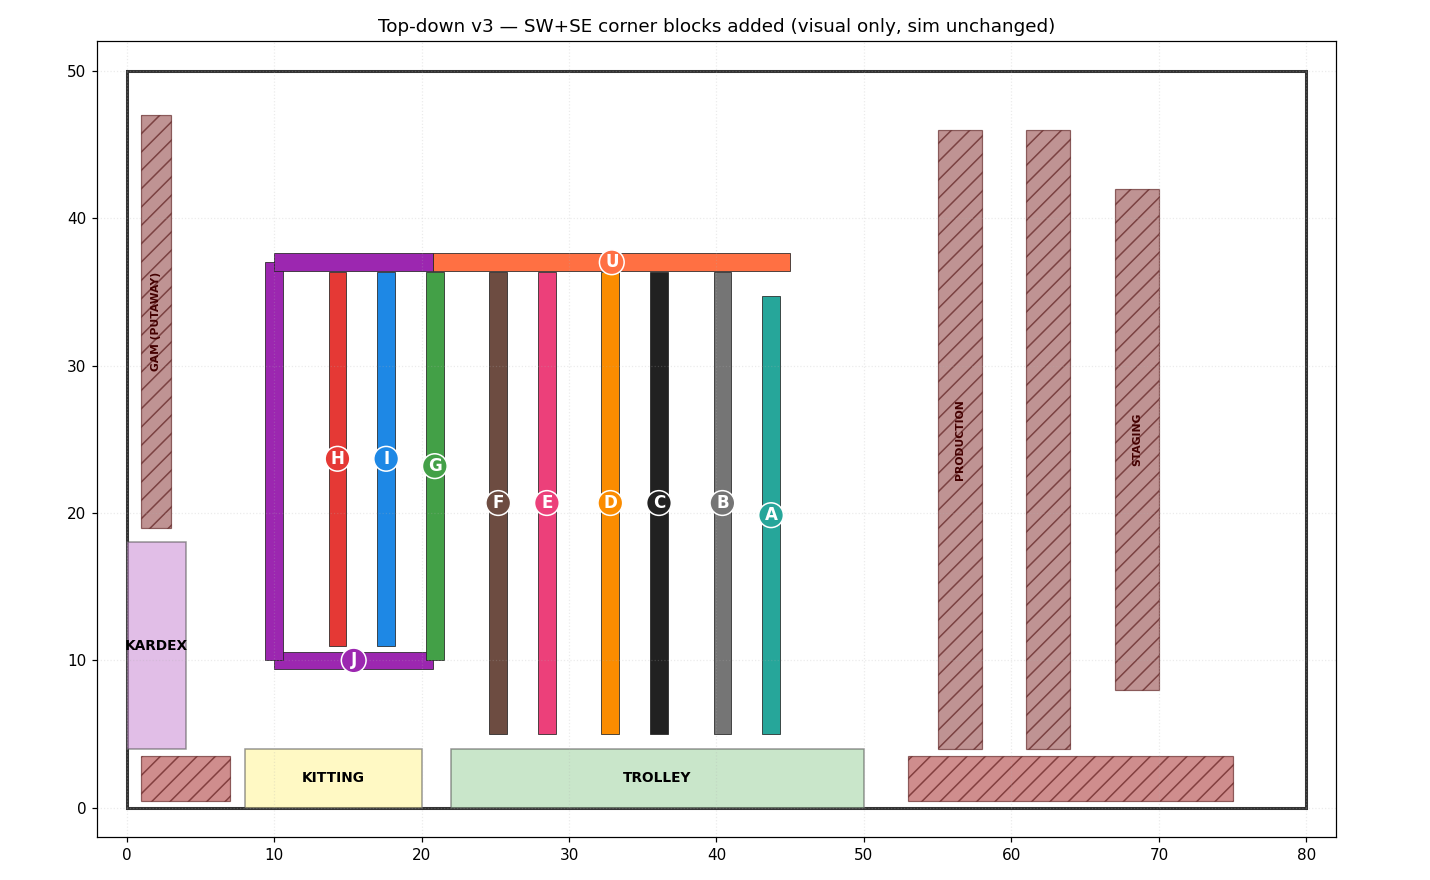
\includegraphics[width=0.92\textwidth]{fig1_layout}
\caption{Top-down layout of the modelled warehouse. Rack rows are labelled A
through J and U; kit corridors (about 2~m) alternate with reach-truck aisles
(about 3~m) along the east-to-west sequence.}
\label{fig:layout}
\end{figure}

% ============================================================ 2 LITERATURE
\section{Literature Review}
This section reviews work across four threads: discrete-event simulation
(DES) in warehousing, warehouse layout optimization with multi-criteria
classification, automated storage and retrieval systems (AS/RS), and decision
support systems (DSS) in warehouse management. It closes by identifying the
research gap that motivates the proposed line-aware slotting policy.

\subsection{Simulation-Based Warehouse Analysis}
Simulation-based approaches are frequently used to evaluate warehouse
performance and capacity-related issues in a comprehensive way.
Discrete-event simulation (DES) makes it possible to analyse complex systems
that involve stochastic arrivals, variable processing times, and constraints
on shared resources. Negahban and Smith~\cite{negahban2014} demonstrate that
simulation is an effective tool for identifying bottlenecks, evaluating
storage utilization, and testing alternative system configurations in both
manufacturing and warehouse environments. Such approaches are particularly
useful for questions like whether the shipment area is large enough or how the
workforce should be allocated, and they can be explored without disrupting the
real operation. Hapsari et al.~\cite{hapsari2025} reach a similar conclusion
for an Indonesian pharmaceutical warehouse, where a discrete-event model
surfaced bottlenecks and inventory-control problems that a static ABC analysis
could not reveal. A recurring limitation, however, is that many studies focus
on a single aspect such as routing or capacity in isolation, whereas a real
warehouse requires an integrated analysis that brings together layout,
routing, and operational decision-making.

\subsection{Warehouse Layout Optimization}
Ardiansyah et al.~\cite{ardiansyah2024} address the operational inefficiencies
in warehouse picking that are caused by unoptimized layouts and irregular
product placement, and they note that picking typically consumes far more time
than checking, packing, or loading. Their case study identifies how
large-volume items, such as expired motorcycle tires, can obstruct forklift
lanes and exceed the racking capacity, which leads to a breakdown of
First-In-First-Out (FIFO) discipline. To resolve these problems, the authors
integrate Double ABC analysis, which classifies inventory by both pickup
frequency and outer volume, with discrete-event simulation built in Arena to
model and validate the outbound process. A one-way ANOVA confirmed a
significant reduction in moving time, showing that the proposed layout reduces
operator travel distance and helps locate the bottlenecks in the system. Their
work provides a mathematically validated framework for optimizing
limited-space warehouses, and it is the methodological basis for the Double
ABC policy evaluated in the present study.

\subsection{Automated Storage and Retrieval Systems (AS/RS)}
Automation technologies such as AS/RS are often proposed to improve warehouse
performance. AS/RS use cranes or robotic systems in high-density racks, which
increases space efficiency and reduces dependence on manual labour. The
literature reports advantages including higher storage density from narrower
aisles, shorter travel time, better accuracy, and safer operation through
reduced human-vehicle interaction. These systems also carry trade-offs,
mainly high investment cost and reduced flexibility~\cite{roodbergen2009}.

AS/RS design involves two parts: physical design and control
policies~\cite{roodbergen2009}. Physical design fixes rack dimensions, aisle
configuration, and density; control policies set the storage-assignment
strategy, such as dedicated, random, or class-based storage. Class-based
storage is widely preferred because it balances accessibility against space
use. Performance is usually judged by travel time, throughput, waiting time,
and resource utilization. AS/RS represents the highest level of physical
automation, but the present study shows that meaningful gains are available
from slotting policy alone, without the capital cost of full automation.

\subsection{Decision Support Systems in Warehouse Management}
Warehouse design, storage location assignment, and order picking are
frequently studied as separate problems, even though in practice they are
closely linked. Moghadam et al.~\cite{moghadam2025} show that treating these
elements independently leads to suboptimal performance, because layout choices
directly determine where items are stored and how efficiently they can be
picked. The present study addresses this by evaluating different storage and
classification policies without physically altering the warehouse layout, an
approach supported by Amorim-Lopes et al.~\cite{amorim2021}, who show that
combining simulation with optimization can yield significant reductions in
travel distance and order-retrieval time even when the physical layout remains
unchanged.

To support such integrated evaluations, decision support systems (DSS) are
increasingly used in warehouse management to drive data-driven decisions and
improve operational efficiency. In one representative case study, a
warehouse-management DSS was developed to analyse operational data and help
managers evaluate alternative scenarios for layout design, material flow, and
resource utilization; by integrating several performance indicators, the
system enabled a systematic assessment of operations and replaced purely
intuitive managerial judgement. The broader literature indicates that
DSS-based approaches improve the visibility of warehouse processes, raise
decision quality, and help reveal hidden inefficiencies in material handling
and storage. These studies, however, tend to emphasize high-level
decision-making frameworks rather than a detailed model of the underlying
operations. Combining the DSS philosophy with analytical methods such as
simulation therefore gives a more complete solution. That is the approach
taken here: the operations are modelled in detail first, which produces a
statistically validated, data-driven basis that could later be integrated into
a broader decision-support framework.

\subsection{Research Gap and Contribution}
The literature covers storage assignment, simulation-based analysis, and
layout improvement extensively, but most studies evaluate materials by
aggregate demand and treat items as independent~\cite{gu2007,limere2012}. In
synchronized, production-driven warehouses, however, material flow is shaped
by the requirements of specific production lines and by kitting: components
are consumed in coordinated sets, so their relative locations directly affect
kit preparation time~\cite{hanson2012,petersen2004}.

These system-specific dependencies are rarely addressed in the reviewed
literature, where classification methods are generally applied in a uniform
way without being adapted to the operational characteristics of a particular
warehouse~\cite{hausman1976,roodbergen2009}. The critical gap, then, does not
lie in the absence of established assignment methods, but in the failure to
adapt and evaluate those methods within a real-world warehouse context that
explicitly accounts for production-line-based consumption variability and
kit-level spatial dependencies.

Addressing this gap, the primary contribution of this study is the development
and evaluation of a dependency-aware classification approach, the proposed
\policy{Line-aware Slotting} policy, assessed against five alternative policies
within a single discrete-event simulation framework. The study examines how
established storage strategies can be adapted in practice to reflect actual
operational realities rather than theoretical aggregate demand. By evaluating
all of the policies against the current baseline under identical demand and
resource conditions, the research provides a statistically validated,
application-oriented methodology~\cite{ardiansyah2024,kokroko2025}. The result
is a scalable approach for reducing waiting waste and improving material
synchronization in complex, production-driven environments, achieved without
any physical layout modification.

% ============================================================ 3 METHODOLOGY
\section{Methodology}
This section describes the framework used to analyse the current operation,
develop alternative storage and classification policies, and evaluate their
impact. The approach is built on historical SAP data, detailed system
modelling, and discrete-event simulation. By replicating the warehouse in
software, the policies are tested under identical, controlled conditions,
which allows a fair comparison against fixed metrics. Figure~\ref{fig:method}
summarizes the five phases of the work.

\begin{figure}[htbp]
\centering
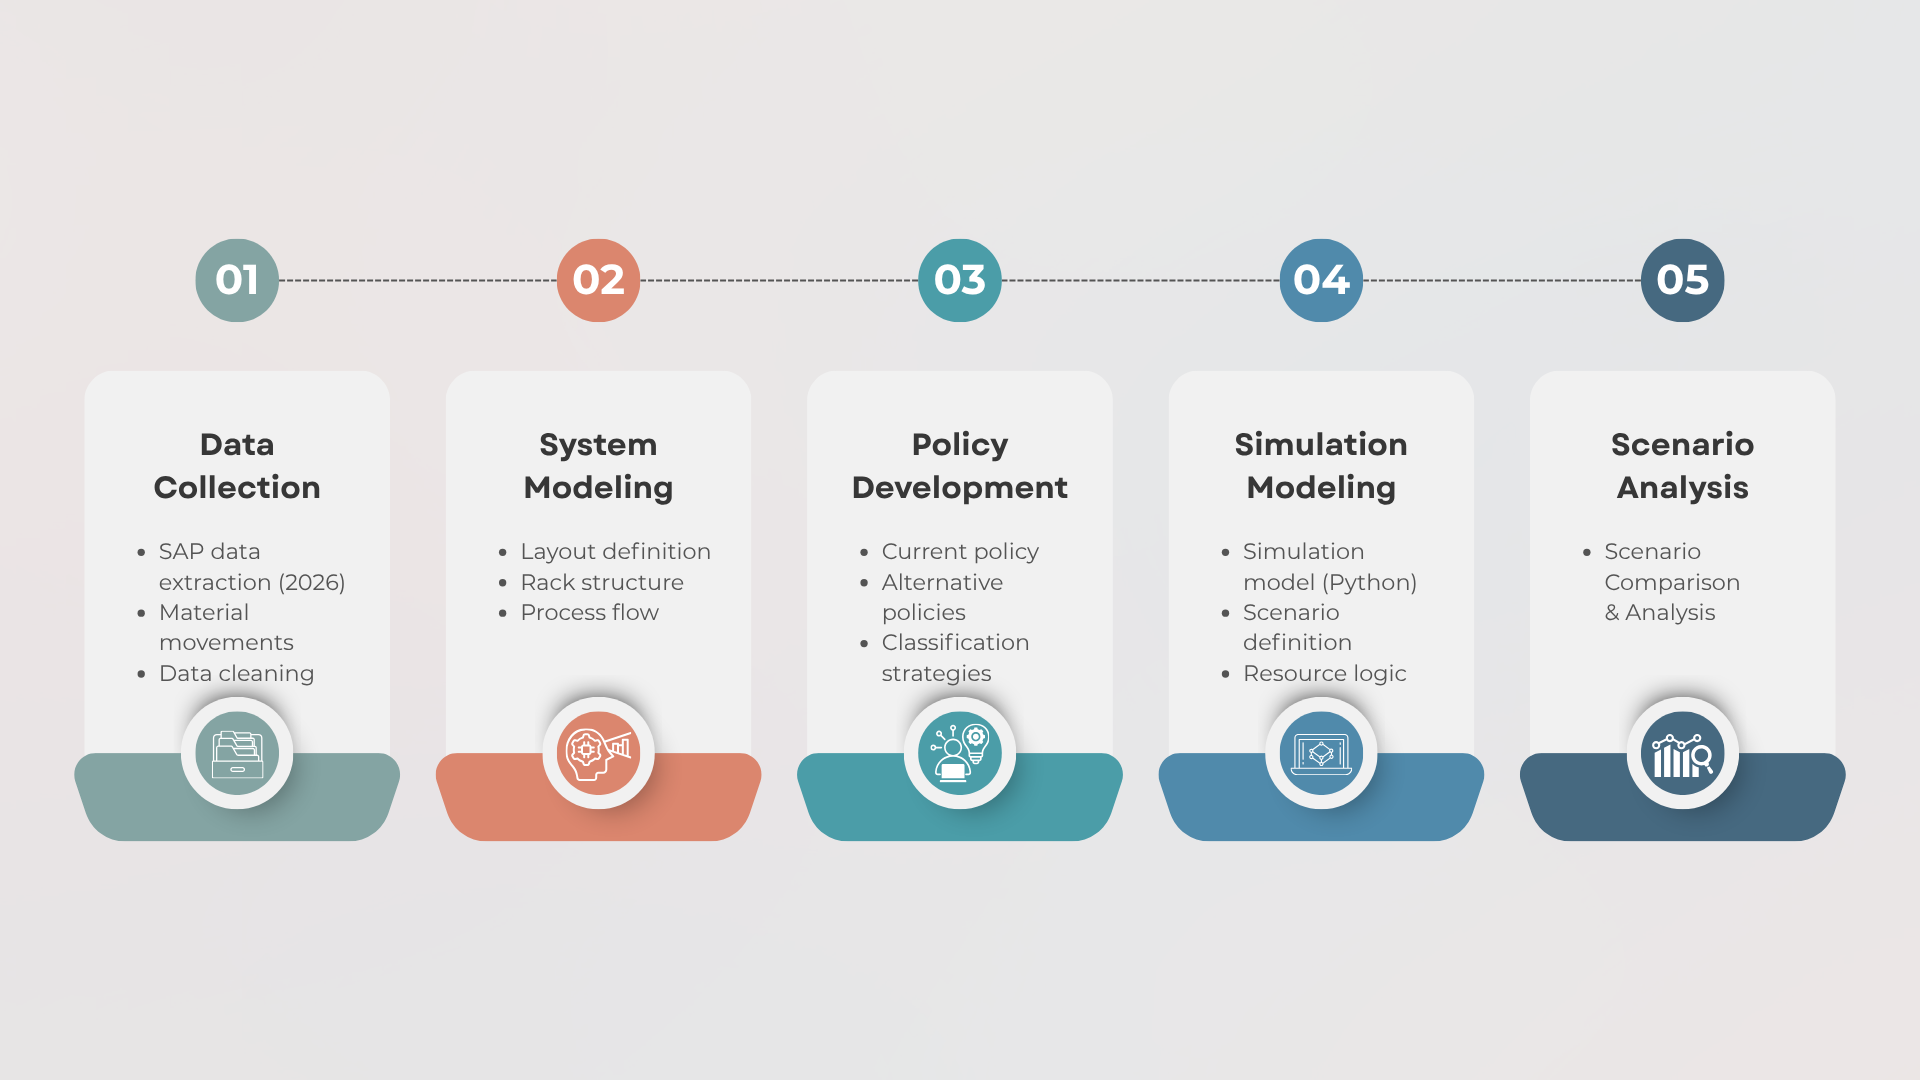
\includegraphics[width=0.95\textwidth]{fig2_methodology}
\caption{The five-phase methodology framework for the simulation-based
warehouse study.}
\label{fig:method}
\end{figure}

\subsection{Data Collection}
The data came directly from the company's SAP system, in cooperation with
company representatives. The analysis uses operational data from 2 January to
18 May 2026, covering 40{,}804 kit orders across 103 active working days.

The primary dataset is the SAP ZWM92 transaction log, which records material
withdrawals, transaction quantities, and the flows associated with kitting and
production support. These records were combined with withdrawal quantities to
determine the actual usage frequency of each component. During preprocessing,
records with zero or negative withdrawal quantities were removed to keep the
dataset clean.

Several supplementary datasets were added: current storage bins, per-line
material usage, and the company's existing ABC/FMR results. An independent
Pareto analysis was carried out on total consumption: materials up to 80\% of
cumulative consumption were classified as A, the next 15\% (to 95\%) as B, and
the remaining 5\% as C~\cite{flores1986,law2015}, as defined in
Equation~\eqref{eq:abc}. This classification was then compared against the
existing one to document differences.

\begin{equation}
\label{eq:abc}
\mathrm{Class}(i)=
\begin{cases}
A, & \text{if } P_i \le 0.80,\\[2pt]
B, & \text{if } 0.80 < P_i \le 0.95,\\[2pt]
C, & \text{if } P_i > 0.95,
\end{cases}
\qquad
P_i=\frac{\sum_{j=1}^{i} c_j}{\sum_{j=1}^{n} c_j},
\end{equation}

\noindent where $c_j$ is the consumption of material $j$ ranked in decreasing
order and $P_i$ is the cumulative consumption share up to rank $i$.

Technical layout drawings and rack documents supplied the physical
dimensions: rack modules, storage levels, fast-mover shelves, aisle widths,
and the relationships between storage and kitting zones. Bill of Materials
(BOM) data and historical kitting records were used to map material
relationships and kit-based usage~\cite{bartholdi2014}.

Beyond the SAP data, operational parameters were collected through field
observation. A video time-motion study recorded 2{,}319 micro-events on the
F400 production line, capturing operator walking speeds, reach-truck movement
and lifting times, manual picking durations, and the operator waiting time
caused by reach-truck dependency. Operator allocation, fast-mover usage,
reachable levels, and handling patterns were recorded as well. Together these
sources formed the quantitative basis for policy development, modelling, and
evaluation.

\subsection{System Modelling}
The warehouse is represented within a discrete-event framework. Storage zones
are modelled as distinct locations; operators and reach trucks (RTs) are
modelled as active resources; the milkrun trains are transport entities; and
production orders are kit-preparation requests triggered by demand.

The physical layout has 11 rack modules with a total capacity of 3{,}203
pallet positions. Materials are unitized on standard Euro pallets
($80 \times 120$~cm). Reach-truck aisles measure 300 to 320~cm and dedicated
kit corridors are 200~cm wide, as confirmed by the facility AutoCAD
measurements. Rack heights reach about 7.5~m, which requires vertical storage
handling~\cite{bartholdi2014}.

A central design feature is the separation between standard storage and
fast-mover sections. The fast-mover zone, the three lowest rack levels up to
about 206~cm, is the manual band, where operators can reach materials without
a reach truck. Here the racks allow decoupled work: operators pick from one
side while replenishment is performed from the other, which removes direct
contact between personnel and equipment. Standard and upper-level positions
require reach-truck support for all retrievals~\cite{roodbergen2009}.

The current state follows a hybrid logic in which assignments are influenced
by line requirements, capacity heuristics, and the existing ABC/FMR
classification. In practice, operations deviate from these rules because of
space limits and immediate replenishment needs, which fragments placement
across zones. This fragmentation adds travel distance, increases reach-truck
dependency, and creates waiting time during kit preparation, especially for
materials in upper levels. The model captures these interactions when
assessing the alternative policies~\cite{gu2007}.

\subsection{Policy Design}
This section describes the storage and classification policies evaluated in
the study. The policies use different elements of the operational data:
physical accessibility, usage frequency, retrieval time, and production-line
and kit dependencies.

\subsubsection{Baseline and Capacity Heuristic (Control Group)}
Two reference policies form the control group:
\begin{itemize}
\item \textbf{Baseline (Actual SAP).} This policy reproduces the historical
placement of the warehouse, reflecting patterns accumulated over years of
operation and daily replenishment. It is the main reference point for
measuring the real-world impact of the alternatives~\cite{kokroko2025}.
\item \textbf{Capacity heuristic.} Materials are assigned to the first
available slot that meets the item's storage requirement, with no line-aware
logic or demand dependency. Comparing the proposed policy against this
heuristic isolates the gain from dependency-aware slotting versus simple space
filling~\cite{roodbergen2009}.
\end{itemize}

\subsubsection{Double ABC Analysis Policy}
The Double ABC policy follows the method of
Ardiansyah et al.~\cite{ardiansyah2024}, which shows that combining two
classification dimensions gives a more granular prioritization than a
single-axis ABC. Because reliable material-volume data were not available,
the second dimension uses material cost rather than volume. The first
dimension captures economic importance (cost) and the second captures
operational importance (frequency). The two criteria are combined in
Table~\ref{tab:doubleabc}.

\begin{table}[htbp]
\centering
\caption{Double ABC classification matrix.}
\label{tab:doubleabc}
\begin{tabular}{lll}
\toprule
Dimension & Classes & Thresholds \\
\midrule
Cost (C) & High / Medium / Low & by unit cost \\
Frequency (F) & High / Medium / Low & $>80\%$ / 80--95\% / 95--100\% cumulative \\
\bottomrule
\end{tabular}
\end{table}

The intersection of the two criteria gives a $3 \times 3$ matrix with nine
categories (AA through CC):
\begin{itemize}
\item \textbf{AA (high cost, high frequency)}: highest priority, assigned to
prime locations such as fast-mover shelves and lower levels.
\item \textbf{CC (low cost, low frequency)}: lowest priority, assigned to
upper levels or less accessible locations.
\item \textbf{Intermediate (AB, BA, and so on)}: placed by their combined cost
and frequency, balancing accessibility against inventory value.
\end{itemize}
This moves the plant beyond simple frequency-based classification and prevents
rack capacity from being consumed by bulky, low-demand items.

\subsubsection{Time-Based Classification Policy}
Unlike static methods based on frequency or volume, the time-based policy uses
the accessibility of each location. In a high-bay warehouse, total retrieval
time is dominated not by horizontal travel but by vertical lift and the need
for reach-truck intervention~\cite{bartholdi2014,heskett1963}. The policy
estimates an access time for each location from travel speed, lift speed, and
reach-truck handling, then assigns frequently used materials to the locations
with the shortest access time. Table~\ref{tab:timebased} summarizes the
mapping. By using time rather than distance alone, the policy aims to reduce
lead time and waiting and to support line synchronization~\cite{petersen2004,limere2012}.

\begin{table}[htbp]
\centering
\caption{Time-based policy: storage zone assignment by access time.}
\label{tab:timebased}
\begin{tabular}{lll}
\toprule
Relative access time & Storage assignment & Access method \\
\midrule
Minimal  & Fast-mover shelves & Manual picking \\
Short    & Lower rack levels  & Reach truck, minimal vertical travel \\
Moderate & Mid rack levels    & Reach truck, standard vertical travel \\
Extended & Upper levels       & Reach truck, significant vertical travel \\
\bottomrule
\end{tabular}
\end{table}

\subsubsection{Line-aware Slotting (Proposed Policy)}
The proposed \policy{Line-aware Slotting} policy is the core contribution of
this study. It shifts the focus from warehouse-wide averages to
production-line dependencies. The implementation has two stages. First, an
independent ABC analysis is run for each production line rather than for the
warehouse as a whole, so materials are ranked by their consumption within each
line, with A-class defined as the top 80\% of cumulative consumption. This
removes the distortion caused by aggregated data and reflects the true
criticality of each material for its line. Second, the policy uses historical
kitting and BOM data to identify items that are frequently picked together and
places them in the same rack module or aisle. Materials shared across several
lines are positioned centrally in high-accessibility zones to reduce
unnecessary travel~\cite{hanson2012,limere2012}.

The placement logic prioritizes the manual band, the three lowest levels that
operators can reach by hand. By keeping high-frequency, line-specific
materials in this zone, the policy achieves two goals at once: proximity, so
materials sit close to the line they serve, and reach-truck decoupling, so
frequent picks no longer require an RT~\cite{dekoster2007}. This directly
attacks the waiting waste in the kit corridors and reduced reach-truck
utilization to 1.3\% in the simulation, as reported in Section~\ref{sec:results}.

\subsection{Simulation Model}
The model was built with the Python SimPy library to represent the
interaction of warehouse operations and to evaluate the alternative policies.
Simulation was chosen because it can capture resource congestion and
stochastic arrivals under realistic conditions without disrupting the real
operation~\cite{gu2007,negahban2014,banks2010}. The implementation is
organized into 17 source modules that handle the full lifecycle: data loading
and SAP ZWM92 bin decoding, warehouse geometry, rectilinear routing with
rack-body obstacles, slotting policy management, the SimPy process logic, KPI
recording, and validation through sensitivity sweeps.
Figure~\ref{fig:lifecycle} shows the lifecycle of one kit order in the model.

\begin{figure}[htbp]
\centering
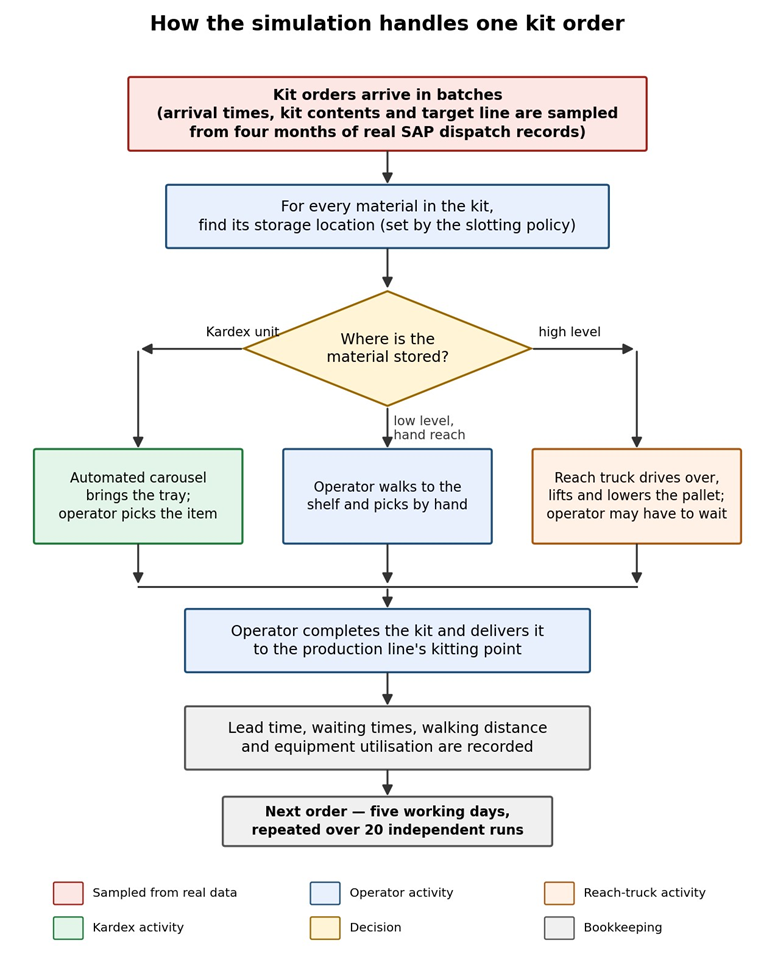
\includegraphics[width=0.78\textwidth]{fig3_lifecycle}
\caption{Lifecycle of a single kit order in the simulation.}
\label{fig:lifecycle}
\end{figure}

Order arrivals are generated from the demand pattern in the SAP ZWM92 log,
using empirical inter-batch gaps and batch sizes. The inter-batch arrival gap
has a mean of 5.36~minutes and a coefficient of variation of 2.04, while the
mean batch size is 4.68 kits. The coefficient of variation of the gap is well
above 1.0, which rules out an exponential model and justifies sampling from
the empirical distribution rather than a fitted theoretical
one~\cite{law2015,simpy}. Service times use lognormal distributions
parameterized from the F400 time-motion study, with a mean operator pick time
of 0.113~minutes, a reach-truck pick-and-place time of 0.110~minutes, a manual
high-level pick penalty of 0.102~minutes, and a Kardex retrieval time of
0.113~minutes. The coefficient of variation is defined in
Equation~\eqref{eq:cv}, and each lognormal distribution is moment-matched to
its measured mean and coefficient of variation through
Equations~\eqref{eq:sigma} and \eqref{eq:mulog}.

\begin{align}
\mathrm{CV} &= \frac{s}{\bar{x}} \label{eq:cv}\\[2pt]
\sigma &= \sqrt{\ln\!\left(1+\mathrm{CV}^{2}\right)} \label{eq:sigma}\\[2pt]
\mu_{\log} &= \ln(\bar{x}) - \tfrac{1}{2}\sigma^{2} \label{eq:mulog}
\end{align}

\noindent where $\bar{x}$ and $s$ are the sample mean and standard deviation
of the measured time, and $\sigma$ and $\mu_{\log}$ are the shape and location
parameters of the lognormal distribution; the location term in
Equation~\eqref{eq:mulog} keeps the distribution mean equal to $\bar{x}$ for
any $\sigma$.

When an order is triggered, the model looks up the storage location of each
requested material, computes the shortest obstacle-free rectilinear travel
path for the assigned resource, and performs the pick. Travel distance uses
the rectilinear (Manhattan) metric of Equation~\eqref{eq:manhattan}, evaluated
between pick points and summed over the route; the router searches a set of
aisle waypoints and returns the shortest path that avoids rack bodies. If a
required resource is busy, the order waits in a queue and the waiting time is
recorded.

\begin{equation}
\label{eq:manhattan}
d(A,B) = \lvert x_A - x_B \rvert + \lvert y_A - y_B \rvert
\end{equation}

The architecture lets the storage-assignment logic be replaced without
changing the rest of the model, so every policy faces the same demand stream
and resource pool, which keeps the comparison fair. To check spatial accuracy,
a 3D viewer was built in Three.js that renders the layout from the AutoCAD DWG
file and the eleven rack PDF drawings. Visual inspection of the exported
movement paths confirmed that agents follow the corridors and do not pass
through rack bodies~\cite{ardiansyah2024,sargent2013}.

\subsection{Performance Metrics}
The policies are evaluated on five key performance indicators (KPIs):
\begin{itemize}
\item \textbf{Kitting lead time (min/order).} Time from order creation until
the completed kit is ready at the staging area for milkrun pickup. Lower lead
time means faster supply to the lines.
\item \textbf{Operator waiting time (min/order).} Time the kitting operator
spends idle, waiting for reach-truck support to retrieve upper-level
materials.
\item \textbf{Reach-truck utilization (\%).} Share of total reach-truck
capacity actively used for retrieval, defined in Equation~\eqref{eq:util}.
\item \textbf{Throughput (orders/day).} Number of kits completed per working
day, defined in Equation~\eqref{eq:thru}.
\item \textbf{Operator walking distance (m/order).} Total rectilinear path
length an operator walks to complete one kit. This metric checks that any lead
time reduction comes from smarter placement, not from making the operator walk
further.
\end{itemize}

\begin{align}
U_{\mathrm{RT}} &= \frac{\sum_{r=1}^{N_{\mathrm{RT}}} t^{\mathrm{busy}}_r}
{T_{\mathrm{sim}}\, N_{\mathrm{RT}}} \label{eq:util}\\[2pt]
\Lambda &= \frac{N_{\mathrm{completed}}}{T_{\mathrm{sim}}} \label{eq:thru}
\end{align}

\noindent where $t^{\mathrm{busy}}_r$ is the busy time of reach truck $r$,
$N_{\mathrm{RT}}$ is the number of reach trucks, $T_{\mathrm{sim}}$ is the
simulated horizon, and $N_{\mathrm{completed}}$ is the number of completed kit
orders.

\subsection{Verification and Validation}
\subsubsection{Verification}
Verification checked that the model was built correctly and behaves as
intended, through code-level checks and logical-flow tests. At the code level,
tests covered the SAP bin decoder, the Kardex routing logic, and resource
tracking. A ten-step control list confirms that the modelled pallet capacity
is consistent with the layout file before any result is recorded, that every
material has a valid location, and that pick counts are correct. The model
checks that its 3{,}101 modelled positions reconcile with the 3{,}203 pallet
positions stated in the rack drawings (the difference reflects narrower feeder
bays and a cart-parking slot) before a run proceeds. Fixed random seeds make
each run exactly reproducible.

The logical flow was then tested step by step, covering order creation,
picking, and reach-truck use. The model was also run on small scenarios whose
expected travel and waiting times could be computed by hand and compared
against the output. Finally, extreme scenarios were tested: with all materials
on the lowest levels the model produced zero reach-truck waiting, and with all
materials on the top levels it produced a clear rise in waiting and reach-truck
use. As Table~\ref{tab:verify} shows, the difference between the hand
calculation and the simulation was below 1\% in every scenario.

\begin{table}[htbp]
\centering
\caption{Verification test outcomes.}
\label{tab:verify}
\begin{tabular}{lll}
\toprule
Test scenario & Expected behaviour & Outcome \\
\midrule
Single lower-rack retrieval & Minimal wait, no RT needed & Pass \\
Single upper-rack retrieval & RT request generated & Pass \\
No upper-rack materials & Near-zero waiting time & Pass ($0.12$~min) \\
All upper-rack materials & High RT use, long wait & Pass \\
\bottomrule
\end{tabular}
\end{table}

To keep the comparison between policies fair, common random numbers (CRN) were
used, so every policy faces the same sequence of orders and any difference
comes from the storage strategy rather than from random variation.

\subsubsection{Validation}
Validation assessed whether the model represents the real warehouse, following
the Sargent framework~\cite{sargent2013} with both operational review and
statistical checks. First, the physical and operational elements, including
the layout, racks, fast-mover areas, and milkrun cycles, were reproduced from
SAP data, drawings, BOM relationships, and field observation, and the process
logic was reviewed with company representatives.

Second, a chi-square goodness-of-fit test compared the simulated pick
distribution against the historical SAP ZWM92 data. The pooled test gave
$\chi^2(7)=535.05$ ($p<0.001$), pooled from the ten-rack restricted test
$\chi^2(9)=537.68$ to satisfy Cochran's rule, with a Cramér's V of 0.22,
which indicates a small-to-medium effect. The statistic and effect size are
defined in Equations~\eqref{eq:chisq} and~\eqref{eq:cramer}. Because the
simulation assigns pick locations using its own logic rather than replaying
history, an exact bin-for-bin match is neither expected nor desired; the rack
ranking, however, agrees, and the busiest racks in the log (E, G, and D) are
also the busiest in the model. Table~\ref{tab:validate} summarizes the checks.

\begin{align}
\chi^2 &= \sum_{i=1}^{k}\frac{(O_i-E_i)^2}{E_i} \label{eq:chisq}\\[2pt]
V &= \sqrt{\frac{\chi^2}{n\,(k-1)}} \label{eq:cramer}
\end{align}

\noindent where $O_i$ and $E_i$ are the observed and expected pick counts in
rack $i$, $k$ is the number of racks, and $n$ is the total number of picks.

\begin{table}[htbp]
\centering
\caption{Validation summary (Sargent framework).}
\label{tab:validate}
\begin{tabular}{lll}
\toprule
Validation check & Result & Key metric \\
\midrule
Distributional fit (chi-square) & Pass (disclosed) & $\chi^2(7)=535.05$, $V=0.22$ \\
Daily volume calibration & Pass & Error $1.1\%$ vs $\approx396$ kits/day \\
Route model (zero crossings) & Pass & No agent crosses a rack body \\
Reproducibility & Pass & Stable across seeds \\
\bottomrule
\end{tabular}
\end{table}

The daily volume calibration matched the real average of about 396 kits per
day within 1.1\%. The routing model was checked on simulated agent paths, with
no agent passing through a rack body. Reproducibility checks confirmed stable
results across seeds. Together these checks support the use of the model for
comparing storage policies.

\subsection{Experimental Design and Statistical Analysis}
\label{sec:expdesign}
Each policy was run for $N=20$ independent replications. Common random numbers
were used across policies: replication $i$ of every policy uses seed
$42+i$ for the arrival stream, so all policies face the same demand
trajectory in a given replication. This pairing removes demand-side variance
from the policy comparison. Within a policy the replications use distinct
seeds and are therefore independent; across policies, the replications are
correlated by design through the shared seeds, which is exactly what the
paired analysis exploits. A warm-up period was excluded from each run to
reduce initialization bias, so only post-warm-up output was retained.

For each replication, the model recorded the mean of each KPI. The sample
mean, standard deviation, and a 95\% confidence interval were then computed
for each policy and KPI. Because $N=20$, the interval uses the
$t$-distribution with 19 degrees of freedom ($t_{0.025,19}=2.093$), as in
Equation~\eqref{eq:ci}.

\begin{equation}
\label{eq:ci}
\bar{x} \pm t_{0.025,\,19}\,\frac{s}{\sqrt{N}}
\end{equation}

A one-way ANOVA was used as the primary test, with storage policy as the
factor (six levels) and the per-replication KPI as the response, at a
significance level of $\alpha=0.05$. Because each KPI is an average of many
events within a replication, its distribution across replications is
approximately normal, and the sample sizes are equal, so the assumptions for
the parametric test are reasonable. The ANOVA statistic is given in
Equation~\eqref{eq:anova} and the hypotheses in Equation~\eqref{eq:anovah}.

\begin{equation}
\label{eq:anova}
F = \frac{\mathrm{MS}_{B}}{\mathrm{MS}_{W}}
  = \frac{\mathrm{SS}_{B}/(k-1)}{\mathrm{SS}_{W}/(N_{\text{tot}}-k)}
\end{equation}

\begin{equation}
\label{eq:anovah}
H_0:\ \mu_1=\mu_2=\cdots=\mu_6
\qquad
H_1:\ \exists\, i\neq j \ \text{such that}\ \mu_i\neq\mu_j
\end{equation}

Where the ANOVA was significant, Tukey's Honestly Significant Difference (HSD)
test identified which pairs differ. In addition, common-random-number paired
$t$-tests compared each alternative directly against the Actual SAP baseline.
The paired test (Equation~\eqref{eq:pairedt}) uses the per-replication
differences, which removes the shared demand variance and gives a tighter
contrast.

\begin{equation}
\label{eq:pairedt}
t = \frac{\bar{d}}{s_d/\sqrt{N}}, \qquad
d_i = \mathrm{KPI}_{\text{alt},i} - \mathrm{KPI}_{\text{base},i}
\end{equation}

\noindent with hypotheses $H_0:\ \mu_d=0$ and $H_1:\ \mu_d\neq0$. A negative
mean difference favours the alternative policy. The KPI values were exported
per replication for the analysis and for cross-checking in Minitab.

% ============================================================ 4 RESULTS
\section{Results and Discussion}
\label{sec:results}
This section reports the simulation results for the six policies.
Section~\ref{sec:res-comp} gives the replication-level KPIs and confidence
intervals, Section~\ref{sec:res-sens} the sensitivity analysis,
Sections~\ref{sec:res-anova} and~\ref{sec:res-paired} the statistical tests,
Section~\ref{sec:res-cohen} the effect size, and Section~\ref{sec:res-disc}
the discussion.

\subsection{Simulation Results and Policy Comparison}
\label{sec:res-comp}
The outputs are stable across the 20 replications. The proposed
\policy{Line-aware Slotting} policy reached a mean kitting lead time of
6.91~minutes with a narrow 95\% confidence interval of $[6.44, 7.38]$. Its
mean operator waiting time was 4.26~minutes, and reach-truck utilization was
only 1.27\%, which is consistent with placing frequently used materials in
hand-reachable positions. Throughput stayed at about 398.6 orders per day, so
the policy improves preparation without reducing output. Tables~\ref{tab:lead}
through~\ref{tab:thru} report lead time, waiting time, reach-truck
utilization, and throughput; Table~\ref{tab:walk} reports walking distance.
Figure~\ref{fig:comparison} compares the policies across four panels.

\begin{table}[htbp]
\centering
\caption{Kitting lead time by policy ($N=20$ replications).}
\label{tab:lead}
\begin{tabular}{lccc}
\toprule
Policy & Mean (min) & Std.\ dev. & 95\% CI \\
\midrule
Line-aware Slotting & 6.91 & 0.99 & $[6.44,\ 7.38]$ \\
Baseline (Actual SAP) & 12.37 & 2.29 & $[11.30,\ 13.44]$ \\
Baseline (Heuristic) & 14.71 & 2.84 & $[13.38,\ 16.04]$ \\
Double ABC & 14.74 & 2.89 & $[13.38,\ 16.09]$ \\
Usage-based ABC & 15.24 & 3.08 & $[13.80,\ 16.68]$ \\
Travel-distance Optimized & 24.60 & 7.19 & $[21.23,\ 27.96]$ \\
\bottomrule
\end{tabular}
\end{table}

\begin{table}[htbp]
\centering
\caption{Operator waiting time by policy ($N=20$ replications).}
\label{tab:wait}
\begin{tabular}{lccc}
\toprule
Policy & Mean (min) & Std.\ dev. & 95\% CI \\
\midrule
Line-aware Slotting & 4.26 & 0.98 & $[3.80,\ 4.72]$ \\
Baseline (Actual SAP) & 8.45 & 2.29 & $[7.38,\ 9.52]$ \\
Baseline (Heuristic) & 10.40 & 2.85 & $[9.07,\ 11.73]$ \\
Double ABC & 10.40 & 2.90 & $[9.04,\ 11.76]$ \\
Usage-based ABC & 10.81 & 3.10 & $[9.37,\ 12.26]$ \\
Travel-distance Optimized & 19.03 & 7.20 & $[15.66,\ 22.40]$ \\
\bottomrule
\end{tabular}
\end{table}

\begin{table}[htbp]
\centering
\caption{Reach-truck utilization by policy ($N=20$ replications).}
\label{tab:util}
\begin{tabular}{lccc}
\toprule
Policy & Mean (\%) & Std.\ dev. & 95\% CI \\
\midrule
Line-aware Slotting & 1.27 & 0.28 & $[1.14,\ 1.40]$ \\
Baseline (Actual SAP) & 21.71 & 2.46 & $[20.55,\ 22.86]$ \\
Baseline (Heuristic) & 22.82 & 2.71 & $[21.55,\ 24.09]$ \\
Double ABC & 24.58 & 2.83 & $[23.25,\ 25.90]$ \\
Usage-based ABC & 24.41 & 2.74 & $[23.12,\ 25.68]$ \\
Travel-distance Optimized & 43.95 & 4.72 & $[41.74,\ 46.16]$ \\
\bottomrule
\end{tabular}
\end{table}

\begin{table}[htbp]
\centering
\caption{Throughput by policy ($N=20$ replications).}
\label{tab:thru}
\begin{tabular}{lccc}
\toprule
Policy & Mean (orders/day) & Std.\ dev. & 95\% CI \\
\midrule
Line-aware Slotting & 398.58 & 44.49 & $[377.76,\ 419.40]$ \\
Baseline (Actual SAP) & 398.51 & 44.45 & $[377.71,\ 419.31]$ \\
Baseline (Heuristic) & 398.38 & 44.31 & $[377.64,\ 419.12]$ \\
Double ABC & 398.39 & 44.29 & $[377.66,\ 419.12]$ \\
Usage-based ABC & 398.42 & 44.42 & $[377.63,\ 419.21]$ \\
Travel-distance Optimized & 396.17 & 43.16 & $[375.98,\ 416.37]$ \\
\bottomrule
\end{tabular}
\end{table}

\begin{table}[htbp]
\centering
\caption{Operator walking distance by policy ($N=20$ replications).}
\label{tab:walk}
\begin{tabular}{lccc}
\toprule
Policy & Mean (m/order) & Std.\ dev. & 95\% CI \\
\midrule
Baseline (Actual SAP) & 89.0 & 1.30 & $[88.4,\ 89.6]$ \\
Line-aware Slotting & 92.4 & 1.79 & $[91.6,\ 93.3]$ \\
Travel-distance Optimized & 96.1 & 1.65 & $[95.3,\ 96.9]$ \\
Double ABC & 104.6 & 1.70 & $[103.8,\ 105.4]$ \\
Baseline (Heuristic) & 106.1 & 1.90 & $[105.2,\ 107.0]$ \\
Usage-based ABC & 108.8 & 1.67 & $[108.0,\ 109.6]$ \\
\bottomrule
\end{tabular}
\end{table}

The walking-distance results in Table~\ref{tab:walk} are central to the
interpretation. \policy{Line-aware Slotting} walks 92.4~m per order, slightly
more than the 89.0~m of the current SAP placement, yet its lead time is about
half. The gain therefore does not come from shorter walking; it comes from
removing reach-truck calls from the kit path, which is examined in
Section~\ref{sec:res-disc}.

\begin{figure}[htbp]
\centering
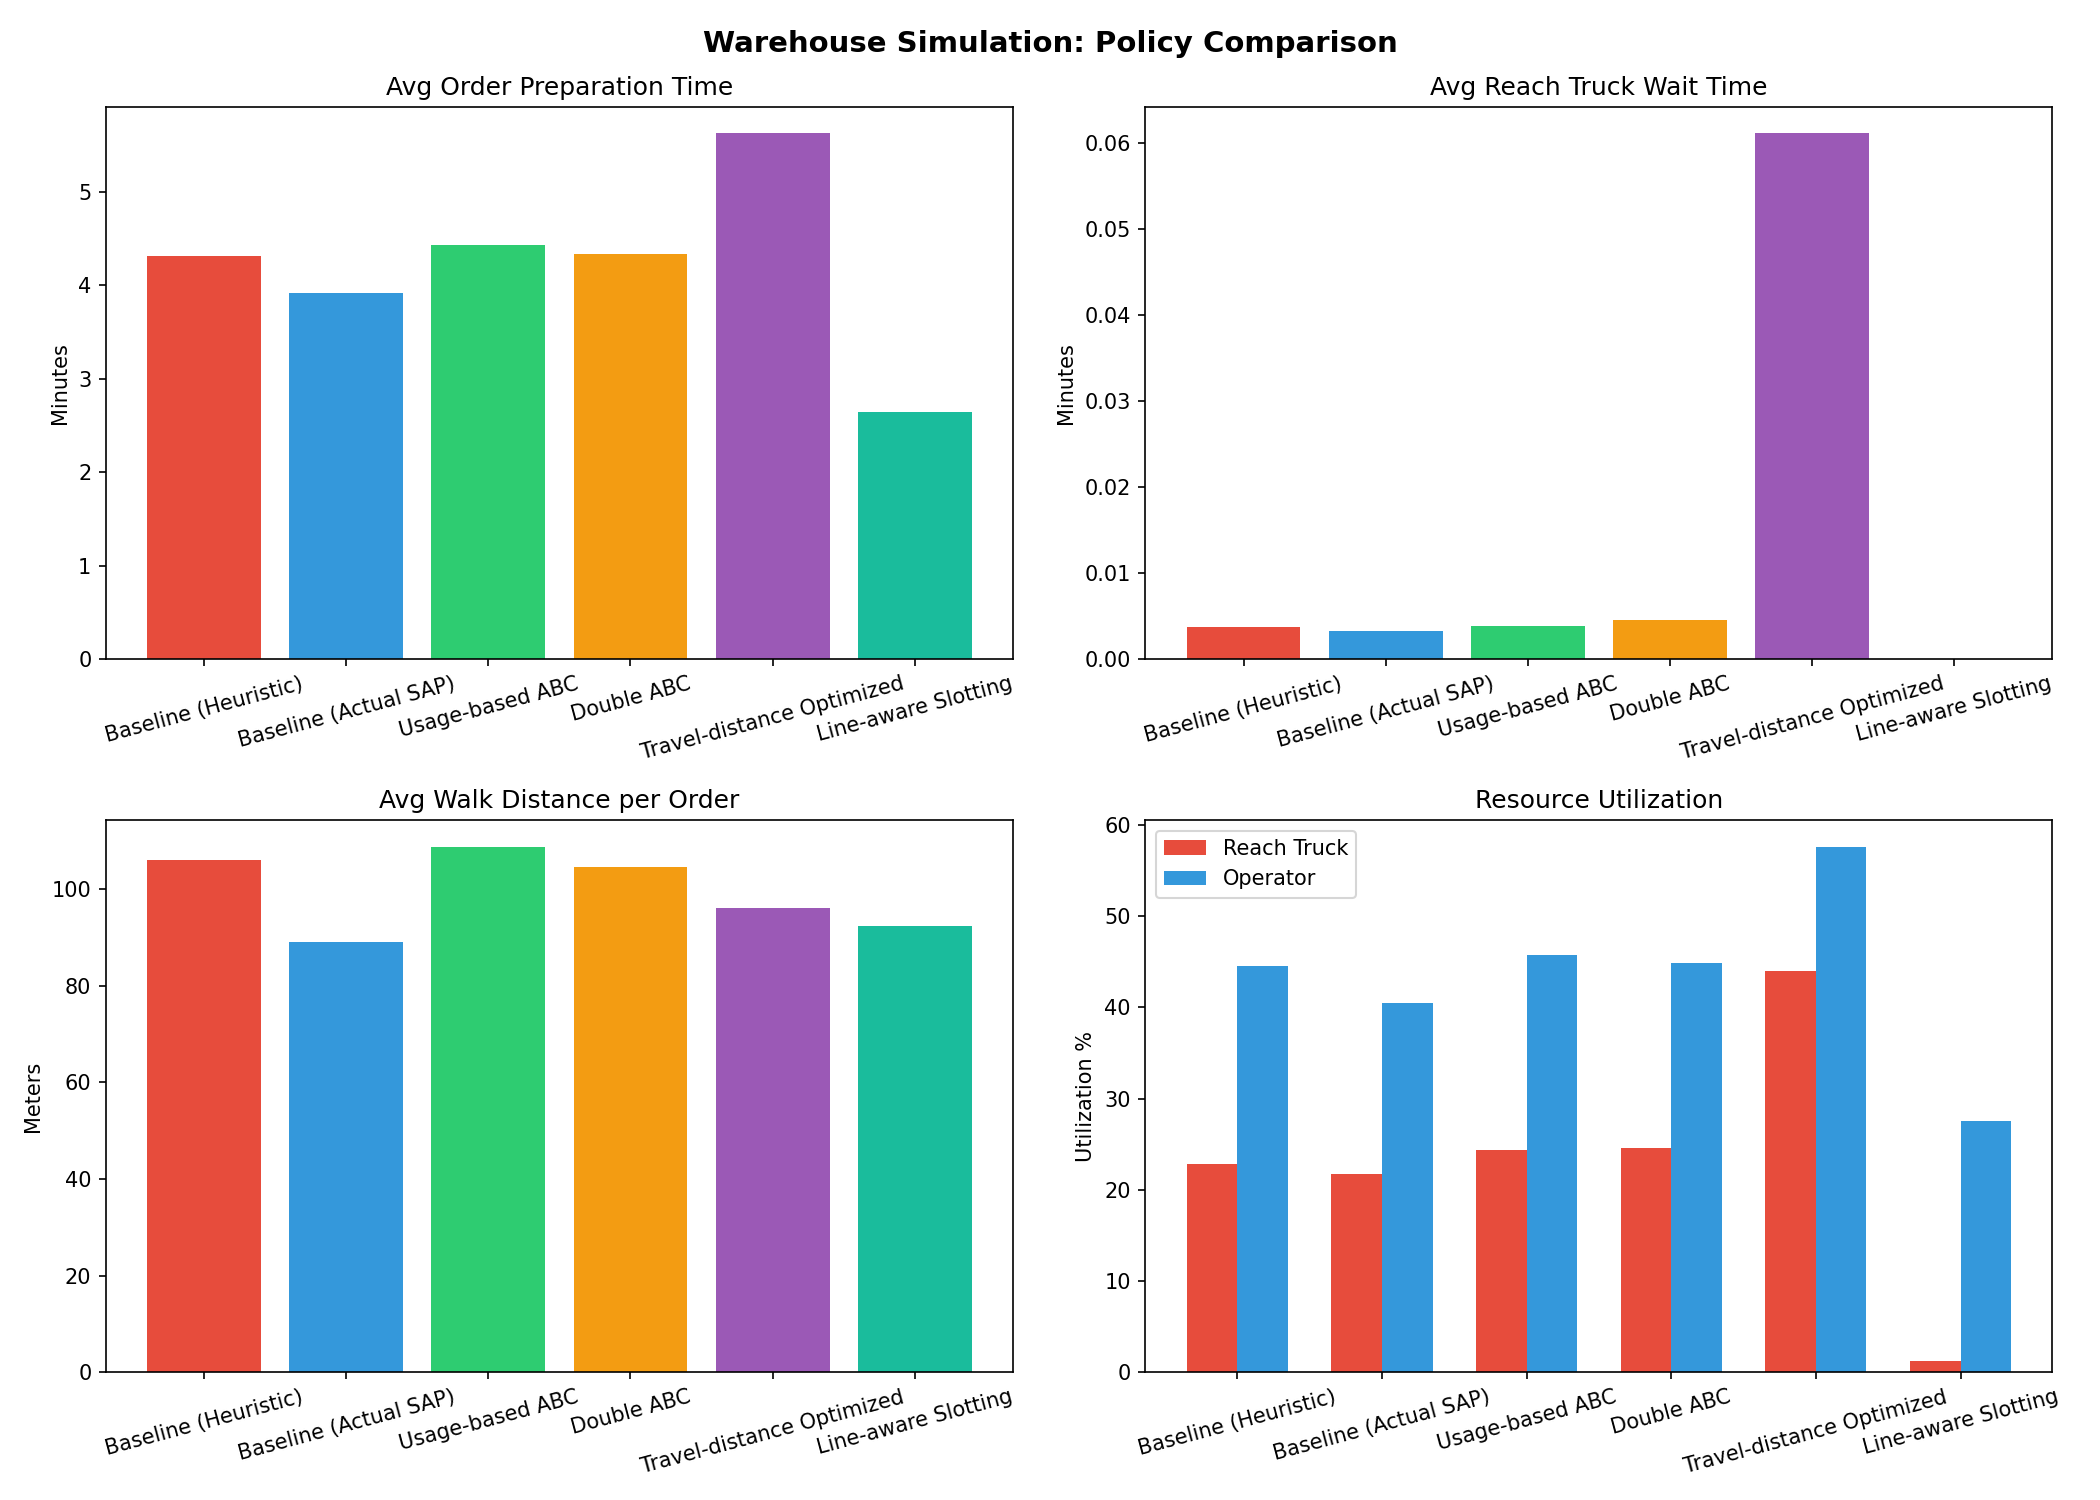
\includegraphics[width=\textwidth]{fig4_comparison}
\caption{Policy comparison across four panels: average order preparation time,
average reach-truck wait time, average walking distance per order, and
resource utilization (reach truck and operator). All values are means over
$N=20$ replications with common random numbers.}
\label{fig:comparison}
\end{figure}

\subsection{Sensitivity Analysis}
\label{sec:res-sens}
A one-at-a-time (OAT) sensitivity analysis was run on nine timing and
operational parameters, using the capacity heuristic as the reference policy
($N=5$ replications per cell, baseline lead time 14.00~minutes). Each
parameter was varied by $\pm20\%$ from its calibrated value while the others
were held constant. Table~\ref{tab:sens} reports the resulting minimum and
maximum lead time and the swing, defined as the range divided by the baseline.

\begin{table}[htbp]
\centering
\caption{One-at-a-time sensitivity of kitting lead time to $\pm20\%$ parameter
changes (capacity heuristic reference, baseline 14.00~min; $\star$ marks a
swing above 15\%).}
\label{tab:sens}
\begin{tabular}{lcccc}
\toprule
Parameter & Base value & Min lead (min) & Max lead (min) & Swing \\
\midrule
Operator walking speed & 50 m/min & 12.03 & 17.40 & 38.3\% $\star$ \\
Order inter-arrival time & 5.36 min & 12.29 & 17.53 & 37.4\% $\star$ \\
Reach-truck lift time per level & 0.25 min & 12.74 & 15.33 & 18.5\% $\star$ \\
Reach-truck travel speed & 100 m/min & 13.65 & 14.58 & 6.6\% \\
Kardex carousel time & 0.40 min & 13.74 & 14.27 & 3.8\% \\
Operator pick time & 0.113 min & 13.79 & 14.21 & 3.0\% \\
Kardex pick time & 0.113 min & 13.82 & 14.19 & 2.6\% \\
Reach-truck pick/place time & 0.110 min & 13.91 & 14.11 & 1.5\% \\
Manual high-level pick penalty & 0.102 min & 13.99 & 14.06 & 0.5\% \\
\bottomrule
\end{tabular}
\end{table}

Lead time is most sensitive to operator walking speed (38.3\% swing) and to
the arrival rate (37.4\%), followed by the reach-truck lift time per level
(18.5\%). The remaining parameters move lead time by less than 7\%. The
conclusions are therefore robust to estimation error in the smaller timing
constants. Figure~\ref{fig:sens} shows the same result as a tornado chart.

\begin{figure}[htbp]
\centering
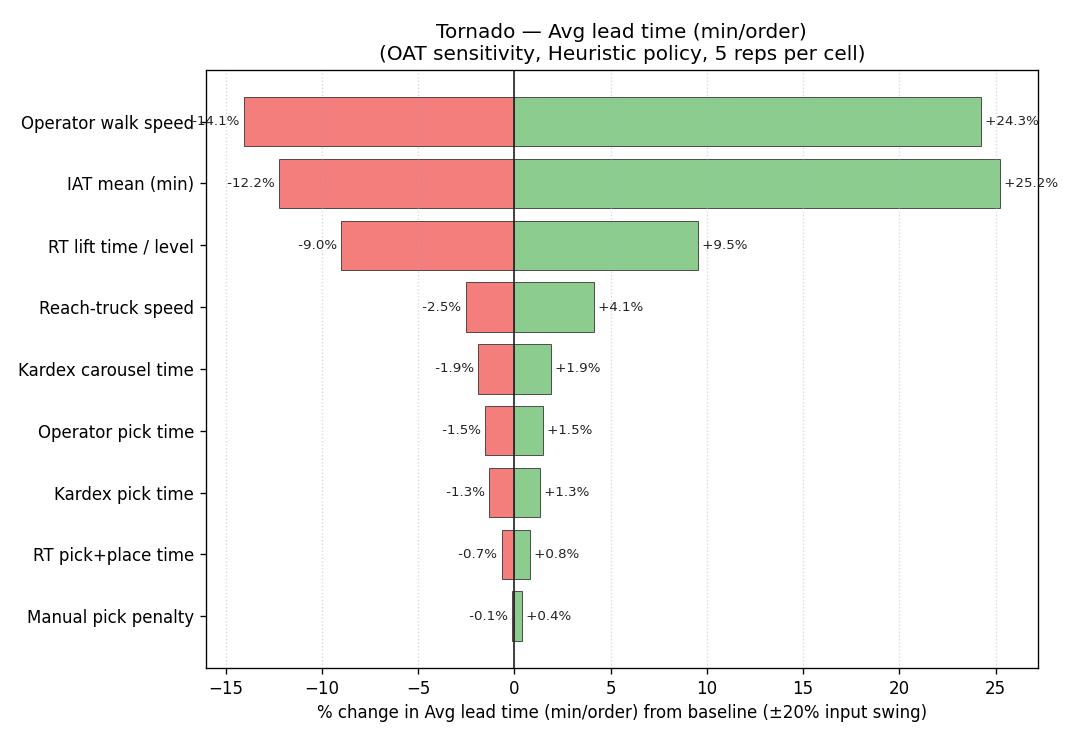
\includegraphics[width=0.85\textwidth]{fig5_sensitivity}
\caption{Tornado chart of the one-at-a-time sensitivity of mean kitting lead
time to $\pm20\%$ changes in each parameter.}
\label{fig:sens}
\end{figure}

A stress test was also run by doubling the arrival rate (twice the system
load). Under this heavier load the lead-time advantage of \policy{Line-aware
Slotting} over the SAP baseline grows from 5.46~minutes at normal load to
20.7~minutes, which shows that the policy becomes more valuable as the system
is pushed harder.

\subsection{Statistical Hypothesis Testing}
\label{sec:res-anova}
The one-way ANOVA (Table~\ref{tab:anova}) shows that the choice of storage
policy has a significant effect on kitting lead time, waiting time,
reach-truck utilization, and walking distance ($p<0.001$ in each case).
Throughput does not differ between policies ($F=0.01$, $p\approx1.0$), which
confirms that the system is not order-constrained: it completes about the same
number of kits per day regardless of policy, so the gains appear as lower lead
time and waiting rather than as higher output.

\begin{table}[htbp]
\centering
\caption{One-way ANOVA across the six policies for each KPI ($N=20$ per
policy). $H_0$: all policy means are equal.}
\label{tab:anova}
\begin{tabular}{lcccl}
\toprule
KPI & $F$ & d.f. & $p$-value & Decision at $\alpha=0.05$ \\
\midrule
Kitting lead time & 47.07 & (5, 114) & $3.55\times10^{-26}$ & Reject $H_0$ \\
Total waiting time & 33.09 & (5, 114) & $9.86\times10^{-21}$ & Reject $H_0$ \\
Reach-truck utilization & 430.06 & (5, 114) & $3.19\times10^{-72}$ & Reject $H_0$ \\
Walking distance & 464.15 & (5, 114) & $5.12\times10^{-74}$ & Reject $H_0$ \\
Throughput & 0.01 & (5, 114) & $1.000$ & Fail to reject $H_0$ \\
\bottomrule
\end{tabular}
\end{table}

\subsection{Paired \texorpdfstring{$t$}{t}-Test Results and Policy Contrast}
\label{sec:res-paired}
Table~\ref{tab:paired} reports the common-random-number paired $t$-tests on
kitting lead time against the current SAP placement. \policy{Line-aware
Slotting} reduces lead time by 5.46~minutes per order ($t=-17.47$,
$p=3.68\times10^{-13}$), and the interval does not approach zero. Every other
alternative is significantly slower than the current state: the capacity
heuristic and the two ABC variants add roughly 2.3 to 2.9~minutes per order,
and the travel-distance policy adds 12.23~minutes.

\begin{table}[htbp]
\centering
\caption{Replication-paired $t$-tests on kitting lead time against the current
SAP placement (common random numbers, $N=20$ pairs). A negative difference
favours the alternative policy.}
\label{tab:paired}
\begin{tabular}{lcccc}
\toprule
Policy vs.\ current placement & Mean diff.\ (min) & $t$ & $p$-value & Significant? \\
\midrule
Capacity heuristic & $+2.34$ & $11.27$ & $7.47\times10^{-10}$ & Yes \\
Usage-based ABC & $+2.87$ & $9.97$ & $5.50\times10^{-9}$ & Yes \\
Double ABC & $+2.37$ & $10.05$ & $4.85\times10^{-9}$ & Yes \\
Travel-distance Optimized & $+12.23$ & $10.06$ & $4.82\times10^{-9}$ & Yes \\
Line-aware Slotting & $-5.46$ & $-17.47$ & $3.68\times10^{-13}$ & Yes \\
\bottomrule
\end{tabular}
\end{table}

The pattern is clear: frequency-based or distance-based slotting alone is not
enough for this warehouse. The drivers of improvement are line-based
accessibility and a reduced dependence on reach trucks. The
\policy{Line-aware Slotting} policy is the only alternative that improves on
the current state, because it considers both the production-line relationship
and the manual accessibility of materials, which lowers reach-truck
intervention and stabilizes the kitting process.

\subsection{Practical Effect Size: Cohen's d}
\label{sec:res-cohen}
ANOVA and the paired $t$-tests establish statistical significance; Cohen's $d$
measures the practical size of the improvement. For the primary contrast,
\policy{Line-aware Slotting} versus the SAP baseline, the effect size is
$d=3.10$ (mean difference 5.46~min, pooled standard deviation 1.76~min), as in
Equation~\eqref{eq:cohen} and Table~\ref{tab:cohen}. Since $d \ge 0.8$ is
conventionally large, a value of 3.10 indicates a very large practical effect,
which confirms that the improvement is operationally meaningful and not just
statistically detectable.

\begin{equation}
\label{eq:cohen}
d = \frac{\bar{x}_1 - \bar{x}_2}{s_p}, \qquad
s_p = \sqrt{\frac{(n_1-1)s_1^2 + (n_2-1)s_2^2}{n_1+n_2-2}}
\end{equation}

\begin{table}[htbp]
\centering
\caption{Cohen's $d$ for the primary policy contrast (benchmarks: $d\ge0.2$
small, $\ge0.5$ medium, $\ge0.8$ large).}
\label{tab:cohen}
\begin{tabular}{lccc}
\toprule
Contrast & Mean diff.\ (min) & Pooled SD (min) & Cohen's $d$ \\
\midrule
Line-aware vs.\ SAP baseline (lead time) & 5.46 & 1.76 & 3.10 \\
\bottomrule
\end{tabular}
\end{table}

\subsection{Discussion}
\label{sec:res-disc}
Storage-assignment research has repeatedly found that good slotting can cut
order-picking travel by 10 to 30\% relative to random or class-based
baselines. The present result is consistent in magnitude, since
\policy{Line-aware Slotting} walks 92.4~m per order against 106.1~m for the
capacity heuristic, a 13\% reduction. It also adds a dimension that the layout
literature rarely emphasizes: in a kitting environment with shared reach
trucks, the dominant benefit of slotting is the reduction of resource
contention rather than of travel distance.

The kitting context is central. A kit order bundles materials from across the
warehouse into one set. Limere et al.~\cite{limere2012} show that the choice
between kitting and line stocking turns on handling cost and distance; this
study shows that when reach trucks are shared, the handling cost is mainly
queueing time. A policy that ignores this turns a resource that is idle about
78\% of the time under SAP placement into one that is saturated at 44\% under
a pure travel-distance policy. Simulation is well suited to expose this
non-linear behaviour, as also noted by
Negahban and Smith~\cite{negahban2014} and Amorim-Lopes et
al.~\cite{amorim2021}.

Three features drive the advantage of \policy{Line-aware Slotting}. First, the
line-origin distance metric places each material near the line it serves most;
because about 77\% of kit demand originates at line-specific corridor points,
this concentrates picks in small neighbourhoods. Second, the preference for
no-reach-truck levels keeps materials at hand height and reserves the fleet
for genuine high-level retrieval. Third, by spreading materials across several
corridor segments, the policy avoids the local congestion that cripples the
travel-distance strategy.

The Usage-based and Double ABC policies both follow the textbook rule to place
fast movers nearest the output point. In a single-picker warehouse this is
sound, but here there is no single dispatch dock: each line has its own
kitting corridor. Collapsing that structure into one distance metric creates
the same congestion as the travel-distance policy, only to a smaller degree.
The travel-distance policy is the extreme case, optimizing the wrong objective
and producing a lead time about double the current state.

For the Manisa plant the implication is direct: re-slot fast movers line by
line, with priority to the levels reachable by hand. At about 400 kit orders
per day, the model estimates a mean reduction of 5.46~minutes per order, which
is a substantial capacity gain over a shift with no new equipment or
headcount. One caveat is that the 1.3\% reach-truck utilization reported for
the proposed policy is a picking-only figure. Putaway and replenishment, which
would rise after moving high-turnover items to lower levels, are outside the
model; quantifying that trade-off is a priority for future work. The
comparison itself is fair, since every policy faces the same demand
trajectory under common random numbers, the same resource pool, and the same
modelling assumptions.

% ============================================================ 5 CONCLUSIONS
\section{Conclusions and Future Work}
\subsection{Conclusions}
This study developed a discrete-event simulation model of the Schneider
Electric Manisa warehouse using historical SAP data, warehouse layout
information, Bill of Materials (BOM) relationships, and operational time
studies. The model was used to evaluate alternative storage-assignment
policies under realistic operating conditions, and it allowed those policies
to be tested without disrupting the ongoing warehouse activity. Six policies
were compared in total: the current SAP placement, a capacity heuristic, two
frequency-based ABC variants, a travel-distance optimizer, and the proposed
\policy{Line-aware Slotting} policy.

The results showed that storage-assignment decisions have a clear and
measurable effect on warehouse performance. Among the evaluated alternatives,
the proposed \policy{Line-aware Slotting} policy achieved the best overall
performance: it reduced mean kitting lead time from 12.37 to 6.91~minutes per
order, an improvement of about 44\%, while reach-truck utilization fell from
21.7\% to 1.3\%. One-way ANOVA and common-random-number paired $t$-tests
confirmed that these improvements are statistically significant and are not an
artefact of simulation randomness, and the very large effect size
($d=3.10$) confirms that the gain is operationally meaningful as well.

The findings indicate that the primary source of inefficiency in the current
system is not travel distance but the operational dependency created by
reach-truck intervention during kit preparation. By positioning frequently
used, line-specific materials within hand-reachable storage, the proposed
policy reduces waiting time, improves the synchronization between the
warehouse and the production lines, and increases overall process efficiency.
Notably, it achieves this even though it walks slightly more per order
(92.4~m versus 89.0~m for the current placement), which underlines that the
lever is queueing rather than distance. Overall, the study demonstrates that a
substantial performance improvement is available from a data-driven
storage-assignment policy alone, without costly physical layout changes or
investment in automation.

\subsection{Managerial Implications}
The results provide practical guidance for warehouse managers who want to
improve operational efficiency with limited investment. The proposed
\policy{Line-aware Slotting} policy can be implemented gradually rather than
all at once, by first identifying the most frequently used materials of each
line and relocating them to manually accessible levels close to the production
lines they support. For a facility that processes about 400 kit orders per
day, the observed reduction in kitting lead time represents a substantial
opportunity to cut waiting waste, improve the utilization of operators and
reach trucks, and increase the stability of the kitting process, which in turn
reduces the risk of a line-feed disruption. Beyond the specific policy, the
simulation framework built in this study is itself a decision-support tool:
alternative storage policies can be evaluated and validated virtually before
any physical change is made, which lowers both the operational risk and the
cost of experimenting on the live warehouse.

\subsection{Limitations}
While the simulation provides a sound framework for evaluating
storage-assignment policies, several modelling choices and scope constraints
should be acknowledged, as they define the boundaries within which the results
should be interpreted.

\textbf{Extrapolation of operational times.} The operational time parameters
were derived from a detailed video time-motion study of 2{,}319 micro-events
conducted specifically on the F400 kitting line, and they were then
extrapolated to the other eight product families. If the F400 line is not
fully representative of slower or faster assembly lines, the lead-time
estimates may deviate accordingly. The sensitivity analysis bounds this risk
quantitatively, but line-specific time studies would further refine the
model's accuracy.

\textbf{Validation data and holdout testing.} The model was both fitted and
validated against the same historical SAP ZWM92 dataset, because complete
historical KPI records were not available for out-of-sample testing. The
goodness-of-fit and daily-volume checks therefore serve as rigorous
internal-consistency tests rather than true holdout validation against an
independent observation period.

\textbf{SAP decoding and multi-bin splits.} Although the model parses the SAP
data accurately, only 750 active materials had fully decoded
rack-bay-position codes, and 386 materials in the dataset occupy multiple
storage bins that the model does not split between forward (active) and
reserve assignments. Consequently, the Actual SAP baseline is best understood
as a highly accurate SAP-plus-heuristic hybrid rather than a pure bin-for-bin
replay of the existing layout.

\textbf{Physical routing constraints.} Physical operator congestion within
shared aisles is not modelled, since agents pass through each other freely in
the simulation. As a result, the model may slightly underestimate total
kitting lead time under the high-load, high-congestion policies, such as the
Travel-distance Optimized policy.

\textbf{Scope limited to order picking.} Most importantly, the scope of the
simulation is restricted to order picking and kitting. The proposed
\policy{Line-aware Slotting} policy concentrates fast-moving materials at lower
levels, which will inevitably increase the putaway and replenishment frequency
for those rack positions. The reported 1.3\% reach-truck utilization for the
proposed policy therefore reflects picking workload only, and the total
reach-truck workload in a live deployment would be higher once replenishment
cycles are included. Potential improvements related to replenishment
scheduling, workforce planning, dynamic routing, and equipment allocation were
intentionally excluded from this study in order to isolate the specific impact
of storage location assignment.

\subsection{Future Work}
This study can be extended in several directions. First, additional time
studies could be carried out across the other production lines to obtain
line-specific operational parameters and further improve the accuracy of the
model. Second, kit-based co-location strategies, which place components that
are frequently picked together in adjacent positions, could be integrated with
the proposed \policy{Line-aware Slotting} approach to reduce the picking travel
within a single order even further. Third, a pilot implementation in a
selected warehouse zone would allow a direct before-and-after comparison of
real operational performance, providing independent validation of the policy.
Finally, the simulation could be combined with optimization techniques such as
mathematical programming or metaheuristics to generate and evaluate improved
storage-assignment strategies automatically rather than by manual policy
design.

\subsection{Sustainable Development}
This study aligns with three of the United Nations Sustainable Development
Goals (SDGs)~\cite{un_sdg}, which shows how operational efficiency can also
support sustainable industrial practice. SDG~9 (Industry, Innovation, and
Infrastructure) is the most direct fit: moving from intuition-based storage
assignment to a data-driven simulation framework is an example of
evidence-based industrial innovation, because it improves the process through
analysis rather than through new equipment, additional capital expenditure, or
facility expansion, which in turn supports resilient and efficient
infrastructure. SDG~12 (Responsible Consumption and Production) applies because
the proposed \policy{Line-aware Slotting} policy makes fuller use of the
storage capacity and material-handling equipment that already exist. By
reducing reach-truck utilization, the system consumes less energy per prepared
kit, and by improving spatial efficiency it can delay or remove the need for a
physical building expansion, which conserves land and construction materials.
SDG~8 (Decent Work and Economic Growth) applies on the operator side: shifting
high-frequency items into the lower manual band reduces the ergonomic strain
associated with mast-elevated retrieval and removes the non-value-added idle
time that operators otherwise spend waiting for a reach truck, which
contributes to a safer and more productive work environment. These are not
transformative global claims; they are concrete, honest improvements that
follow directly from the findings of the model.

% ============================================================ REFERENCES
\begin{thebibliography}{99}
\bibitem{amorim2021} M.~Amorim-Lopes, L.~Guimar\~aes, J.~Alves, and B.~Almada-Lobo, ``Improving picking performance at a large retailer warehouse by combining probabilistic simulation, optimization, and discrete-event simulation,'' \textit{International Transactions in Operational Research}, vol.~28, no.~2, pp.~687--715, 2021.
\bibitem{ardiansyah2024} D.~P.~Ardiansyah, F.~A.~O.~Reynaldi, and D.~L.~Widaningrum, ``Improving warehouse layout effectiveness and process picking efficiency with the discrete event system simulation approach,'' \textit{Procedia Computer Science}, vol.~234, pp.~1753--1760, 2024.
\bibitem{banks2010} J.~Banks, J.~S.~Carson, B.~L.~Nelson, and D.~M.~Nicol, \textit{Discrete-Event System Simulation}, 5th ed. Upper Saddle River, NJ: Pearson, 2010.
\bibitem{bartholdi2014} J.~J.~Bartholdi and S.~T.~Hackman, \textit{Warehouse \& Distribution Science}, Release 0.96. Atlanta, GA: Georgia Institute of Technology, 2014.
\bibitem{dekoster2007} R.~de~Koster, T.~Le-Duc, and K.~J.~Roodbergen, ``Design and control of warehouse order picking: a literature review,'' \textit{European Journal of Operational Research}, vol.~182, no.~2, pp.~481--501, 2007.
\bibitem{emde2012} S.~Emde and N.~Boysen, ``Optimally routing and scheduling tow trains for JIT-supply of mixed-model assembly lines,'' \textit{European Journal of Operational Research}, vol.~217, no.~2, pp.~287--299, 2012.
\bibitem{moghadam2025} M.~Farhadi Moghadam, K.~Khalili Damghani, V.~Ghezavati, and A.~Rashidi Komijan, ``A bi-level optimization method for integrated warehouse design, storage location assignment, and order picking,'' \textit{MethodsX}, vol.~15, art.~103595, 2025.
\bibitem{flores1986} B.~E.~Flores and D.~C.~Whybark, ``Multiple criteria ABC analysis,'' \textit{International Journal of Operations \& Production Management}, vol.~6, no.~3, pp.~38--46, 1986.
\bibitem{frazelle2002} E.~Frazelle, \textit{World-Class Warehousing and Material Handling}. New York, NY: McGraw-Hill, 2002.
\bibitem{gu2007} J.~Gu, M.~Goetschalckx, and L.~F.~McGinnis, ``Research on warehouse operation: a comprehensive review,'' \textit{European Journal of Operational Research}, vol.~177, no.~1, pp.~1--21, 2007.
\bibitem{hanson2012} R.~Hanson and L.~Medbo, ``Kitting and time efficiency in manual assembly,'' \textit{International Journal of Production Research}, vol.~50, no.~4, pp.~1115--1125, 2012.
\bibitem{hapsari2025} I.~Hapsari, J.~A.~Arlianto, and P.~Santoso, ``Simulation-based enhancement of warehouse layout and inventory control in an Indonesian pharmaceutical manufacturer,'' \textit{Jurnal Aplikasi Bisnis dan Manajemen}, vol.~11, no.~2, p.~457, 2025.
\bibitem{hausman1976} W.~H.~Hausman, L.~B.~Schwarz, and S.~C.~Graves, ``Optimal storage assignment in automatic warehousing systems,'' \textit{Management Science}, vol.~22, no.~6, pp.~629--638, 1976.
\bibitem{heskett1963} J.~L.~Heskett, ``Cube-per-order index -- a key to warehouse stock location,'' \textit{Transportation and Distribution Management}, vol.~3, pp.~27--31, 1963.
\bibitem{kokroko2025} B.~Y.~Kokroko, J.~Kobi, and E.~K.~Yeboah, ``Warehouse layout design: maximization of storage efficiency and minimization of travel distances using simulation models and optimization algorithms,'' \textit{International Journal of Innovative Science and Research Technology}, vol.~10, no.~10, pp.~3236--3280, 2025.
\bibitem{law2015} A.~M.~Law, \textit{Simulation Modeling and Analysis}, 5th ed. New York, NY: McGraw-Hill, 2015.
\bibitem{limere2012} V.~Limere, H.~Van Landeghem, M.~Goetschalckx, E.-H.~Aghezzaf, and L.~F.~McGinnis, ``Optimising part feeding in the automotive assembly industry: deciding between kitting and line stocking,'' \textit{International Journal of Production Research}, vol.~50, no.~15, pp.~4046--4060, 2012.
\bibitem{negahban2014} A.~Negahban and J.~S.~Smith, ``Simulation for manufacturing system design and operation: literature review and analysis,'' \textit{Journal of Manufacturing Systems}, vol.~33, no.~2, pp.~241--261, 2014.
\bibitem{petersen2004} C.~G.~Petersen and G.~Aase, ``A comparison of picking, storage, and routing policies in manual order picking,'' \textit{International Journal of Production Economics}, vol.~92, no.~1, pp.~11--19, 2004.
\bibitem{roodbergen2009} K.~J.~Roodbergen and I.~F.~A.~Vis, ``A survey of literature on automated storage and retrieval systems,'' \textit{European Journal of Operational Research}, vol.~194, no.~2, pp.~343--362, 2009.
\bibitem{sargent2013} R.~G.~Sargent, ``Verification and validation of simulation models,'' \textit{Journal of Simulation}, vol.~7, no.~1, pp.~12--24, 2013.
\bibitem{simpy} Team SimPy, ``SimPy: discrete-event simulation for Python,'' simpy.readthedocs.io, accessed 10~June 2026.
\bibitem{un_sdg} United Nations, ``The 17 Goals -- Sustainable Development,'' sdgs.un.org/goals, accessed 10~June 2026.
\end{thebibliography}

% ============================================================ APPENDIX
\appendix
\section{Abbreviations and Nomenclature}
\begin{table}[htbp]
\centering
\caption{Abbreviations used in the report.}
\label{tab:abbrev}
\begin{tabular}{ll}
\toprule
Abbreviation & Meaning \\
\midrule
ABC & Activity-based classification (A/B/C demand classes) \\
ANOVA & Analysis of variance \\
BOM & Bill of materials \\
CRN & Common random numbers \\
CV & Coefficient of variation \\
DES & Discrete-event simulation \\
EPT & Electric pallet truck \\
FMR & Fast/medium/rare-mover classification \\
IAT & Inter-arrival time \\
KPI & Key performance indicator \\
OAT & One-at-a-time (sensitivity) \\
RT & Reach truck \\
SAP & Enterprise resource planning system of the plant \\
ZWM92 & SAP warehouse-management dispatch transaction log \\
\bottomrule
\end{tabular}
\end{table}

\section{Full KPI Table}
Table~\ref{tab:kpifull} reports the mean of every KPI over the $N=20$
replications for all six policies, as a single reference.

\begin{table}[htbp]
\centering
\caption{Full KPI table, means over $N=20$ replications.}
\label{tab:kpifull}
\scriptsize
\setlength{\tabcolsep}{3pt}
\begin{tabular}{l*{6}{c}}
\toprule
KPI & \makecell{Current\\SAP} & \makecell{Capacity\\heuristic} & \makecell{Usage\\ABC} & \makecell{Double\\ABC} & \makecell{Travel-dist.\\opt.} & \makecell{Line-aware\\slotting} \\
\midrule
Lead time (min) & 12.37 & 14.71 & 15.24 & 14.74 & 24.60 & 6.91 \\
Prep time (min) & 3.92 & 4.31 & 4.43 & 4.34 & 5.62 & 2.65 \\
Total wait (min) & 8.45 & 10.40 & 10.82 & 10.40 & 19.03 & 4.26 \\
P95 lead time (min) & 35.9 & 43.0 & 42.9 & 41.9 & 70.6 & 18.8 \\
Walk distance (m) & 89.0 & 106.1 & 108.8 & 104.6 & 96.1 & 92.4 \\
Throughput (orders/day) & 398.5 & 398.4 & 398.4 & 398.4 & 396.2 & 398.6 \\
RT utilization & 0.217 & 0.228 & 0.244 & 0.246 & 0.440 & 0.013 \\
Operator utilization & 0.405 & 0.446 & 0.457 & 0.448 & 0.576 & 0.275 \\
Kardex utilization & 0.079 & 0.079 & 0.079 & 0.078 & 0.078 & 0.079 \\
Orders completed (5 days) & 1943 & 1942 & 1942 & 1942 & 1931 & 1943 \\
\bottomrule
\end{tabular}
\end{table}

\end{document}
